\documentclass[../main.tex]{subfiles}
\begin{document}
    \chapter{Research Context}\label{ch:inference_design_context}

	This chapter describes our type system of PHP the research context.
    In section \ref{sec:types} we will explain more about the types we have defined.
    The relation between the types are described in \ref{sec:type_hierarchie}.
    Section \ref{ch:inference_design_context} explains in which context the research is executed.
    
	\section{Types}\label{sec:types}
	The basis types in PHP are integers, floats, booleans, strings, arrays, resources and null.
	PHP has a similar class inheritance structure and interface implementation as Java.
    The main difference is that in PHP all class are \texttt{public} and that inner classes are not allowed in PHP. 
    \\
	Because PHP has no explicit type system, we have defined our own type system for PHP.
	In the Rascal code below you can see our defined types, with a brief description below.
	\begin{program}
    \begin{rascal}
\CAT{Keyword}{module} lang::php::m3::TypeSymbol
 
\CAT{Keyword}{data} TypeSymbol
  = \textbackslash{}any()\footnotemark                         \CAT{Comment}{// unknown, can be any of the types below}
  | arrayType(TypeSymbol arrayType) \CAT{Comment}{// array of a type, can be nested}
  | booleanType()                   \CAT{Comment}{// boolean values}
  | classType(\CAT{Keyword}{loc} decl)             \CAT{Comment}{// a specific class}
  | floatType()                     \CAT{Comment}{// float, double or real}
  | integerType()                   \CAT{Comment}{// integer numbers}
  | interfaceType(\CAT{Keyword}{loc} decl)         \CAT{Comment}{// a specific interface}
  | numberType()                    \CAT{Comment}{// a float or integer}
  | nullType()                      \CAT{Comment}{// empty or undefined value}
  | objectType()                    \CAT{Comment}{// any class type}
  | resourceType()                  \CAT{Comment}{// a build-in type}
  | scalarType()                    \CAT{Comment}{// any number, string, resource or }
  | stringType()                    \CAT{Comment}{// text values}
  ; 
    \end{rascal}
\footnotetext{any is escaped with a backslash because it is a reserved keyword.}      
	\caption{$M^3$ core definitions in Rascal}
	\label{fig:rascal_typesymbols}
	\end{program} 
    
    \paragraph{any} 
    As you can see in the comments in the code above, \ref{fig:rascal_typesymbols}, \texttt{any()} represents the combination of all possible types. 
    This type will be used for mixed and unknown types, for example when variables are used, but are never defined.
    
    \paragraph{arrayType}
    The type \texttt{arrayType(TypeSymbol arrayType)} is a recursive declaration.
    The argument of the type is the type of the array. 
    For example, an array of strings is declared as \texttt{arrayType(stringType())} and for an unknown array the type is \texttt{arrayType(\textbackslash{}any())}.
    
    \paragraph{booleanType}
    The type \texttt{booleanType()} is the type for boolean values.
    Just like any other language the boolean values are \texttt{true} and \texttt{false}.
    
    \paragraph{classType}
    The type \texttt{classType(loc decl)} represents a specific class, or the generic type.
    The argument is the declaration, which represents the logical name of the class. 
    An example of the \texttt{Exception} class is \texttt{classType(|php+class:///exception|)}.
    
    \paragraph{floatType}
    Floating point numbers, also known as floats, reals, and doubles are defined by the \texttt{floatType()}.
    Example are \texttt{1.234}, \texttt{1.2e3}, and \texttt{7E-10}.
    
    \paragraph{integerType}
    Integers are whole numbers in decimal, hexadecimal, octal or binary notation.
    The \texttt{integerType} values can be positive or negative.
    
    \paragraph{interfaceType}
    The \texttt{interfaceType()} represents a specific interface, or the parent interface.
    Interfaces can be provided as type hints.
    
    \paragraph{numberType}
    The type \texttt{numberType()} covers the \texttt{integerType} and \texttt{floatType}.
    Because of coercion, these types can be easily mixed.
    
    \paragraph{nullType}
    The type \texttt{nullType()} is used for the value \texttt{null}.
    
    \paragraph{objectType}
    The type \texttt{objectType()} is the parent type for all class types.
    This type represent the object type and could also been written as \texttt{classType(|php+class:///object|)}.
    
    \paragraph{resourceType}
    The type \texttt{resourceType()} represents the build-in PHP resource type.
    Various function return the resourceType from build-in PHP functions.
    
    \paragraph{scalarType}
    The type \texttt{scalarType()} is the generic type for \texttt{resourceType}, \texttt{booleanType}, \texttt{numberType}, and \texttt{stringType}.
    
    \paragraph{stringType}
    The type \texttt{stringType} represents strings, a sequence of characters.
    
    
    \section{Type hierarchie}\label{sec:type_hierarchie}
    
    The relation between the types is shown in figure \ref{fig:type_hierarchie}.
    In this diagram the \texttt{-Type} postfix is omitted to save space.
    We speak of \textbf{subtypes} when the types are descendant of the given type.
    The subtypes of the root node \texttt{any} are \texttt{scalarType}, \texttt{arrayType}, and \texttt{objectType}.
    
    \begin{figure}[H]
        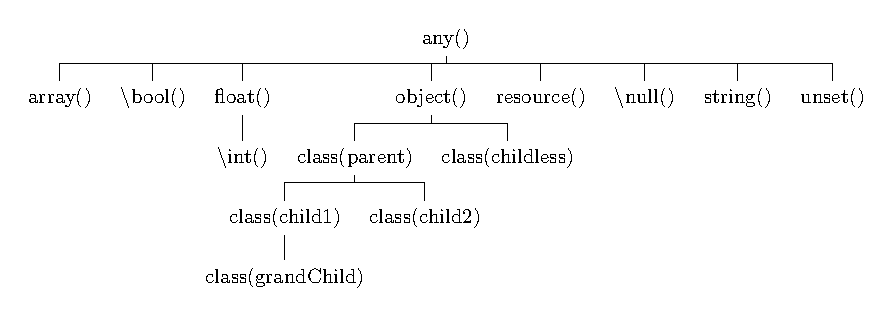
\includegraphics{Diagrams/Subtypes.pdf}
        \caption{Type hierarchy}
        \label{fig:type_hierarchie}
    \end{figure}
    

    The \textit{scalar type} is the super type for the non-complex types \texttt{resourceType}, \texttt{booleanType}, \texttt{numberTypes}, and \texttt{stringType}.
    These types can in practise be combined because of coercion.
    If they are used together, they will be classified as scalar types.
    
	The \textit{array type} in the subtype diagram is the most generic type of array, the array of any type.
	We have omitted the other array types because we of the scope in our research on arrays.
	In theory, this array type is a recursive type and can go to infinite depth.
	But in practise the generic array type is sufficient. 
 
    % show three images next to each other
    \begin{figure}[H]
    \begin{subfigure}[b]{.33\textwidth}
      \begin{center}
      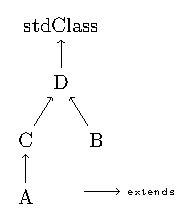
\includegraphics[scale=1]{Diagrams/Inheritance_example.pdf}
      \caption{Inheritance relation}
      \label{fig:subtype}
      \end{center}
    \end{subfigure}
    \begin{subfigure}[b]{.33\textwidth}
      \begin{center}
      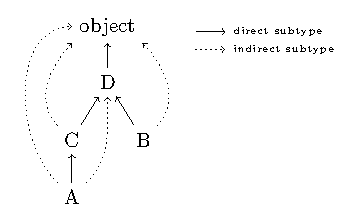
\includegraphics[scale=1]{Diagrams/Subtypes_example.pdf}
      \caption{Subtype relation}
      \label{subtype_tc}
      \end{center}
    \end{subfigure}
    \begin{subfigure}[b]{.33\textwidth}
      \begin{center}
      \lstinputlisting[nolol=true,xleftmargin=20pt,xrightmargin=20pt,language=PHP]{src/php/inheritance.php}
      \caption{Inheritance in PHP}
      \label{subtype_code}
      \end{center}
    \end{subfigure}
    \caption{Relation of subtypes among classes}
    \label{fig:subtypes_classes}
    \end{figure}

	The \textit{object type} is the most generic object type, which represents the \texttt{stdClass} in PHP.
    The class inheritance relation in PHP is a \gls{reflexive transitive closure} relation.
    A class extension of \textbf{\texttt{class A}} on \textbf{\texttt{class C}} will define \textbf{\texttt{class A}} as a subtype of \textbf{\texttt{class C}} in our analysis, as you can see in figure \ref{fig:subtypes_classes}.
    If a class does not extend another class, it will implicitly extend the \gls{stdClass} class.
    You can see that this happens with \textbf{\texttt{class D}} in the example.
    The \textbf{\texttt{stdClass}} is represented as the type \textbf{\texttt{object()}} in our analysis.

    \section{Research context}\label{sec:implementation_context}
    In order to let our research take place, we need to make sure that some environment variables are constant.
    
    \paragraph{Program correctness}
    In order to be able to execute this research we assume that the programs are correct and works as intended.
    This is needed to be able to say something about the programs we analyse.
    
    \paragraph{File includes}
    In this research we will assume that all file are included during runtime. 
    When a PHP system is constructed of classes with namespaces, the files will be logically loaded using PHP's autoloader.
    Because most recent systems use namespaces, we will assume that all files are included.
    For legacy systems, this can influence the results of this research.
    
    \paragraph{Register globals}
    Register globals allows variables to be magically be created from GET and POST values.
    Since it is discouraged to use this setting, we will assume that all software products have this setting disabled.
    
    \paragraph{PHP warnings}
    For this research we will ignore all warnings.
    Warnings do not alter the behaviour of the program.
    In a most production environment these warnings are suppressed and will not change the behaviour of the program.
    
    \paragraph{Flow insensitive}
    % todo check this
    Our analysis is intra-procedural flow insensitive, which means that we don't take the order of statements into account within a function or method scope.
    We do assume type consistency within a scope.
        
\end{document}
